\section{Method}

\begin{figure}[t] 
    \centering
    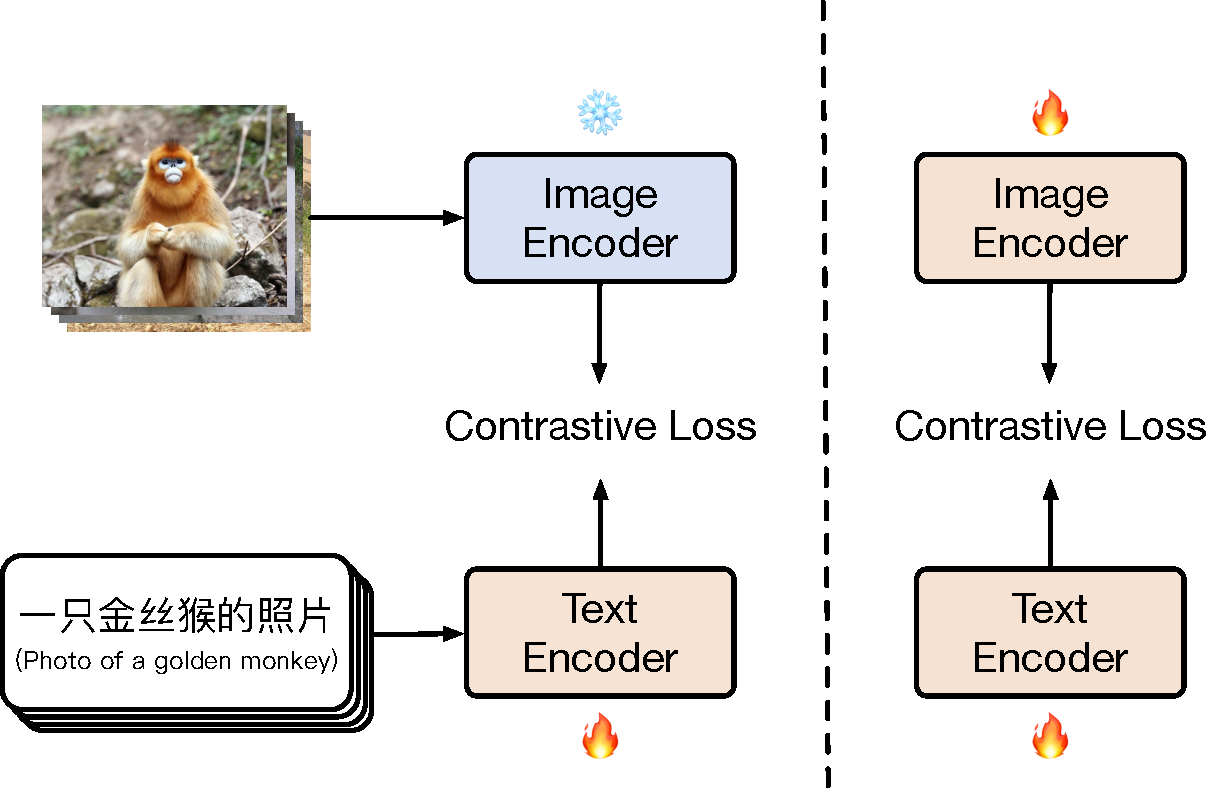
\includegraphics[width=1.0\linewidth]{pics/chinese-clip-model-v3.pdf}
    \caption{\textbf{An illustration of pretraining Chinese CLIP.} To leverage the advantages of the existing pretrained models, we initialize the image encoder with the OpenAI CLIP models, and the text encoder with the Chinese RoBERTa models. In Stage 1, we freeze the weights of the image encoder to avoid weight optimization, and in Stage 2, we unfreeze it and optimize both encoders. }
    \label{fig:model}
\end{figure}

CLIP~\citep{clip} based on simple vision-language contrastive pretraining on large-scale weakly supervised data is a significant foundation model in multimodal representation learning. It can transfer to cross-modal retrieval directly, and its image encoder can play as a vision backbone. 
In this work, we propose to build a language-specific CLIP model by pretraining a vision-language model on large-scale Chinese multimodal data. 
In the following, we provide the details of method design and implementation of our Chinese CLIP. 
% In this section, we first introduce the preliminaries about CLIP and illustrate the details of the data construction and the implementation of Chinese CLIP. 

% \subsection{Preliminaries}

% Before introducing our implementation, we first demonstrate the architecture and training methods of CLIP. 
% CLIP consists of a classical two-tower architecture with an image encoder and a text encoder. 
% An image encoder $\mathcal{M}_{i}$ can be a vision backbone, e.g., ResNet~\cite{resnet}, ViT~\cite{vit}, etc., and a text encoder can be a Transformer model, e.g., BERT~\citep{bert}, GPT~\citep{gpt}, etc. 
% In practice, \citet{clip} proposed CLIP models of multiple model scales with different vision and language backbones. 
% The vision backbones include $5$ ResNets and $3$ ViTs. The $5$ ResNets include ResNet-50, ResNet101, RN50x4, RN50x16, and RN50x64, and the 3 Transformers include ViT-B/32, ViT-B/16, and ViT-L/14. 
% The attention-pooled representation of the top-level features from ResNets or the top-level feature at the $[CLS]$ position from ViTs is treated as the image representation. The top-level feature at the $[EOS]$ position from Transformer is treated as the text representation. 
% To train the model, \citet{clip} applied large-batch contrastive learning. 
% Given $N$ samples in a batch, we have $N \times N$ possible image-text pairs, where there are $N$ positive samples and $N^2 - N$ negative samples. 
% Thus we have $N^2$ similarity scores with inner products of the L2-normalized features and optimize the cross-entropy loss with a learned temperature to control the softmax distribution. 
% CLIP can transfer to cross-modal retrieval directly, and its image encoder can play as a vision backbone. 
%  to replace the original ResNets or ViTs trained on ImageNet~\citep{imagenet}. 
% Furthermore, while CLIP builds a connection between vision and language, it is possible to implement open-vocabulary zero-shot classification by computing similarities between the given image and the candidate labels equipped with a template, e.g., ``a photo of [label]''. To level up the performance in zero-shot image classification, it is a common practice to apply multiple templates to transform a label to multiple sentences, and calculate the mean of the scores of the sentences for a single label. This is also known as prompt ensembling. 

\subsection{Data}
One key to CLIP's success should be the large-scale dataset for pretraining. 
Based on the experiments of a CLIP reimplementation~\citep{openclip}, scaling up data and lengthening the training process can consistently improve the model performance in zero-shot learning. 
This year, the most recent multimodal pretrained models Wukong~\citep{wukong} and R2D2~\citep{r2d2} were pretrained on a public dataset of $100$ million image-text pairs and an in-house dataset of $250$ million samples, where only a subset of $23$ million samples were released. 
For the facility in reimplementation, we aim at pretraining Chinese CLIP on as many publicly available data as possible, and thus we focus on collecting high-quality public datasets. 
We extract the Chinese data (with the mark ``zh'') from the latest LAION-5B~\cite{schuhmann2021laion}, and collect the data from the Wukong dataset. 
However, due to the problems of unavailable links, we can only collect around $108$ million samples and $72$ million samples from LAION-5B and Wukong respectively. 
We additionally add the translated data from the classic English multimodal datasets, including Visual Genome~\cite{vg} and MSCOCO~\citep{coco_cap}, where test sets are removed. 
Finally, we construct a dataset for Chinese multimodal pretraining with around $200$ million image-text pairs.\footnote{We add around $20$ million high-quality internal image-text pairs to provide more diversity. } 
% Furthermore, we add around $20$ million high-quality internal image-text pairs to provide more diversity. 

Below illustrates the procedure for data preprocessing. 
For the part of data from LAION-5B, we remove the samples with CLIP scores lower than $0.26$ computed by mCLIP~\citep{mclip}. 
Besides, we remove the samples with captions containing words in our internal blacklist. 
The blacklist contains words related to advertising, image filenames, etc. 
We remove those samples that are too short (fewer than $5$ characters) or too long (more than $50$ characters). 
For the images, we resize them to the resolution of $224 \times 224$ for most cases and $336 \times 336$ for the ViT-L/14@336px. 

\subsection{Pretraining Method}
\label{subsec:pretraining_method}

There are multiple design choices for pretraining the Chinese CLIP models. 
One of the simplest methods should be pretraining from scratch, where both the image and text encoders are randomly initialized. 
However, we assume that its performance will be limited by the quantity and quality of the current pretraining data. 
To leverage the advantages of existent pretrained models, we initialize the models with weights from the pretrained checkpoints from the official release of CLIP~\footnote{\url{https://github.com/openai/CLIP} License: MIT.} for the image encoder, and RoBERTa-wwm-ext and RBT3~\footnote{\url{https://github.com/ymcui/Chinese-BERT-wwm} License: Apache 2.0} for the text encoder. 
To adapt the model to the introduced pretraining data, it is available to pretrain it with ``contrastive tuning'', similar to the way to transfer CLIP to downstream retrieval data. 
In comparison with contrastive tuning, Locked-image Tuning (LiT)~\citep{lit} demonstrated improved performance in downstream transfer. 

In this work, we propose a two-stage pretraining method, as shown in Figure~\ref{fig:model}. 
The core idea is to first utilize LiT to enable the text encoder to read out high-quality representations from the foundation vision model from OpenAI CLIP, and then transfer the whole model to the domain of the introduced pretraining data. 
It is not sufficient to pretrain Chinese CLIP with solely LiT, as the image encoder should learn the information of the images of the Chinese datasets and model the distribution of such data. 
Before the two-stage pretraining, we first initialize both encoders with pretrained models. 
In Stage 1, we ``lock'' the image encoder by freezing its parameters during pretraining. 
We only pretrain the text encoder for vision-language alignment, based on the assumption that the vision backbone with pretrained weights is already a powerful vision foundation model~\citep{lit, wukong}. 
We pretrain it until there is no salient performance improvement in downstream tasks, even if we prolong the pretraining progress. 
Then we switch to Stage 2, where we ``unlock'' the image encoder by enabling its optimization. 
In Stage 2, we continue pretraining without any parameter frozen, so that the image encoder can learn to model the distribution of the image data from Chinese websites. 
In the ablation study, we discuss the influence of the initialization of the pretrained checkpoints and pretraining methods on the downstream performance. 
Experimental results show that the two-stage pretraining method can outperform either pretraining from scratch or directly finetuning from the pretrained models. 


% \subsection{Scaling}
% \label{subsec:scaling}
% We develop $5$ Chinese CLIP models of different sizes, spanning from around $77$ to $958$ million parameters. 
% We include $1$ ResNet-50 model $\text{CN-CLIP}\rm_{RN50}$ and $4$ ViT models, i.e., $\text{CN-CLIP}\rm_{ViT\text{-}B/16}$, $\text{CN-CLIP}\rm_{ViT\text{-}L/14}$, $\text{CN-CLIP}\rm_{ViT\text{-}L/14@336px}$ and $\text{CN-CLIP}\rm_{ViT\text{-}H/14}$, where models are pretrained on images of the resolution of $224 \times 224$ without specification. 
% Table~\ref{tb:modelcard} presents the details of the model architecture. 
% The smallest model $\text{CN-CLIP}\rm_{RN50}$ consists of a ResNet-50 for the image encoder and a RBT3 for the text encoder. 
% The base-size model $\text{CN-CLIP}\rm_{ViT\text{-}B/16}$ consists of a ViT-B/16@224px for the image encoder and a RoBERTa-wwm-Base for the text encoder. 
% The large-size model $\text{CN-CLIP}\rm_{ViT\text{-}L/14}$ consists of a ViT-L/14@224px for the image encoder and a RoBERTa-wwm-Base for the text encoder, while $\text{CN-CLIP}\rm_{ViT\text{-}L/14@336px}$ consists of a ViT-L/14@336px and a RoBERTa-wwm-Base. 
% Specifically, we pretrain $\text{CN-CLIP}\rm_{ViT\text{-}L/14@336px}$ by continuing pretraining on the pretrained $\text{CN-CLIP}\rm_{ViT\text{-}L/14}$. 
% For the adaptation to a larger resolution, we initialize the image positional embedding by applying interpolation to the positional embedding of $\text{CN-CLIP}\rm_{ViT\text{-}L/14}$, following \citet{openclip}. 
% The huge-size model $\text{CN-CLIP}\rm_{ViT\text{-}H/14}$ consists of a ViT-H/14 for the image encoder and RoBERTa-wwm-Large for the text encoder. 
% More implementation details are presented in Appendix~\ref{sec:implementation_details}.

% \begin{table*}[t]
\center
\small
\vskip 0.15in
\begin{adjustbox}{max width=1.\textwidth}
\begin{tabular}{@{\extracolsep{\fill}}lcccccc}
\toprule
  Model
  & \#Params (All)
  & Backbone (I)
  & \#Params (I)
  & Backbone (T)
  & \#Params (T)
  & Resolution
  \\
\midrule
    $\text{CN-CLIP}\rm_{RN50}$
    & 77M & ResNet-50 & 38M & RBT3 & 39M & $224\times224$
    \\
    $\text{CN-CLIP}\rm_{ViT\text{-}B/16}$
    & 188M & ViT-B/16 & 86M & RoBERTa-wwm-Base & 102M & $224\times224$
    \\
    $\text{CN-CLIP}\rm_{ViT\text{-}L/14}$
    & 406M & ViT-L/14 & 304M & RoBERTa-wwm-Base & 102M & $224\times224$
    \\
    $\text{CN-CLIP}\rm_{ViT\text{-}L/14@336px}$
    & 407M & ViT-L/14 & 304M & RoBERTa-wwm-Base & 102M & $336\times336$
    \\
    $\text{CN-CLIP}\rm_{ViT\text{-}H/14}$
    & 958M & ViT-H/14 & 632M & RoBERTa-wwm-Large & 326M & $224\times224$
    \\
\bottomrule
\end{tabular}
\end{adjustbox}
\caption{Hyperparameters of Chinese CLIP models of different sizes. }
\label{tb:modelcard}
\end{table*}
